\begin{center} 
\emph{``We can never obtain peace in the outer world until we make peace with ourselves.'' -- Dalai Lama}
\end{center}

\section{Outer Products}\label{sec:outer}
We have already discussed some special families of matrices, e.g. nonsingular, elementary, diagonal, and triangular matrices. In this section, we will explore some more special types of matrices and some of their properties. These matrices are important in our study of orthogonality and later when we study eigenvalues.\\

\begin{Def} A real matrix $A$ is \textbf{symmetric} if $A^\top  = A$. A complex matrix $A$ is \textbf{Hermitian} if $A^*=A$.\end{Def}\vs

\begin{Exam} Let $A = \mtx{ccc}{1&2&3\\2&4&5\\3&5&6} $ and $B = \mtx{ccc}{1 & i & 1+i \\ -i & -5 & 2-i \\ 1-i & 2+i & 3}$.  Since $A^\top=A$ and $B^*=B$ (convince yourself!)%Note that 
%\[A^\top = \mtx{ccc}{1&2&3\\2&4&5\\3&5&6}\quad\text{and}\quad B^* =  \mtx{ccc}{1 & i & 1+i \\ -i & -5 & 2-i \\ 1-i & 2+i & 3}. \]
, $A$ is a symmetric matrix and $B$ is an Hermitian matrix.
\end{Exam}\vs

The theory of symmetric and Hermitian matrices is almost identical. We will primarily focus on real matrices below and will only specify Hermitian matrices when a critical difference arises.\\

\begin{Thm} If $A$ and $B$ are $n\times n$ symmetric (Hermitian) matrices and $r\in \R$ ($r\in \C$), then
\begin{multicols}{2}
\begin{enumerate}[!THM!, start =1]
\item $A+B$ is symmetric (Hermitian)\\
\item $rA$ is symmetric (Hermitian)\\
\item $AB$ is symmetric (Hermitian) if and only if $AB=BA$\\
\item if $A$ is invertible, then $A^{-1}$ is symmetric (Hermitian).
\end{enumerate}
\end{multicols}
\end{Thm}%\vspace{-0.25 in}
%\begin{proof}
%The first two statements are straightforward. For (c), note that $(AB)^\top = B^\top A^\top=BA$, since $A$ and $B$ are symmetric. Thus, $AB = BA$ if and only if $AB = (AB)^\top$. This give (c).\\
%
%Suppose that $A$ is invertible. Then $(A^{-1})^\top = (A^\top)^{-1} = A^{-1}$, since $A$ is symmetric. Therefore, $A^{-1}$ is symmetric. This proves (d).
%\end{proof}

\begin{Thm} For any matrix $A$, the matrices $A^\top A$ and $AA^\top$ are symmetric ($A^*A$ and $AA^*$ are Hermitian).
\end{Thm}
%\begin{proof}
%Note that
%\[(A^\top A)^\top = A^\top(A^\top)^\top = A^\top A.\] Thus, $A^\top A$ is symmetric. A similar argument shows that $(AA^\top)^\top = AA^\top$.
%\end{proof}

\begin{Exam} Let $A= \mtx{rrr}{1&-2&4\\3&0&-5}$. Then 
\[A^\top A =  \mtx{rr}{1&3\\-2&0\\4&-5}\mtx{rrr}{1&-2&4\\3&0&-5}= \mtx{rrr}{10&-2&-11\\-2&4&-8\\-11&-8&41}\]
and
\[AA^\top = \mtx{rrr}{1&-2&4\\3&0&-5}\mtx{rr}{1&3\\-2&0\\4&-5} = \mtx{rr}{21&-17\\-17&34}. \qedhere\]
\end{Exam}\vs

\begin{Def} Let $P : F^n\to F^n$ be a linear transformation. We say that $P$ is a \textbf{projection} if $P\circ P = P$.\\

 Let $A$ be the standard matrix of $P$. Then the property that $P\circ P = P$ translate to mean that $A^2=A$. Any matrix (necessarily a square) which satisfies this identity is called an \textbf{idempotent} matrix and is necessarily the standard matrix of a projection.
\end{Def}\vs

Let $\bb x\in F^n$. Then $\bb y = P(\bb x)$ is an arbitrary element of the range of $P$. By definition, we have that 
\[P(\bb y) = P(P(\bb x)) = P\circ P(\bb x) = P(\bb x) = \bb y,\] that is, a projection is exactly a linear transformation that fixes its image. Essentially this means that while some of the coordinates of $\bb x$ are unaltered the other coordinates are forgotten. \\

\begin{multicols}{2}
Geometrically, a projection is a map from the ambient space which projects onto some subspace (the range of the projection). In the process of projecting into the subspace, some information about the vectors is removed so that they can fit inside the smaller space. 
The image of a vector $\bb v$ is the shadow cast by $\bb v$ onto the subspace associated with the projection $P$.\\\

\begin{center}
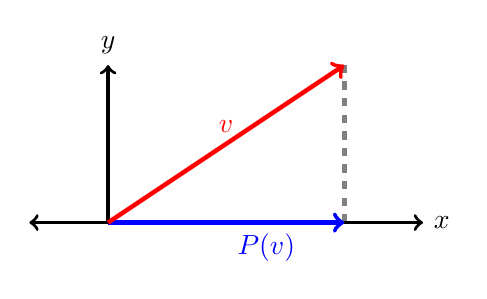
\begin{tikzpicture}
%\draw[dashed, ultra thick, gray] (0,2) -- (3,2);
\draw[dashed, ultra thick, gray] (3,0) -- (3,2);
\draw[->, very thick] (0,0) -- (0,2) node[above] {$y$};
\draw[<->, very thick] (-1,0) -- (4,0) node[right] {$x$};
\draw[->, ultra thick, blue] (0,0) -- (3,0) node[midway, below right] {$\bb P(\bb v)$};
%\draw[->, ultra thick] (0,0) -- (0,2) node[midway, above left] {$\bb v_y$};
\draw[->, ultra thick, red] (0,0) -- (3,2) node[midway, above] {$\bb v$};
\end{tikzpicture}
\end{center}
\end{multicols}

\begin{Exam} For example, the matrices \[\mtx{rr}{1&0\\0&0},\quad \mtx{rrr}{0&0&0\\0&1&0\\0&0&0},\quad \mtx{rrr}{1&0&0\\0&1&0\\0&0&0}\] are easily seen to be idempotent matrices and hence correspond to projections. The first matrix is the projection in $\R^2$ onto the $x$-axis where the $y$-coordinate is forgotten and replaced with 0. Any point already on the $x$-axis has the form $(x,0)$ and is unaffected by the projection.\\

The second matrix is a projection in $\R^3$ onto the $y$-axis, where the $x$- and $z$-coordinates are discarded. Likewise, the third matrix is a projection in $\R^3$ onto the $xy$-plane, where the $z$-coordinate is the only information forgotten. In either case, elements already in the subspace are not altered by the projection.
\end{Exam}\vs

\begin{Exam} The matrices
\[\mtx{rr}{2&2\\-1&-1}, \mtx{rrr}{-8&4&1\\-18&9&2\\0&0&1}\] are also idempotent matrices. (Convince yourself of this). The first matrix corresponds to projection of $\R^2$ onto the line spanned by $(2,-1)$, that is, the line $y=-\dfrac{1}{2}x$. The second matrix corresponds to projection of  $\R^3$ onto the plane spanned by $(4,9,0)$ and $(1,2,1)$, that is, the plane $9x-4y-z=0$. 
\end{Exam}\vs

If $A$ is idempotent, then multiplication by $A$ is projection onto $\col(A)$.\\

%Other than the analogs of the idempotent matrices mentioned in the previous example, the outer product of two vectors can be used to create projections.\\

\begin{Def} Let $\bb u = \mtx{c}{u_1\\\vdots\\u_n}, \bb v = \mtx{c}{v_1\\\vdots\\v_n} \in F^n$. Then the \textbf{outer product} (or \textbf{matrix product})  of $\bb u$ and $\bb v$, denoted $\bb u \otimes \bb v$, is the $n\times n$ matrix of the form $\mtx{c}{u_iv_j}$.
\end{Def}\vs

More compactly, we have that $\bb u \otimes \bb v= \bb u\bb v^\top$ (or $\bb u \otimes \bb v = \bb u\bb v^*$ for complex vectors). This highly resembles the definition of the inner product  $\bb u \cdot \bb v = \bb u^\top \bb v$ (or $\bb u^*\bb v$ for complex vectors). Despite this similarity, the outer product is a matrix and the inner product is a scalar. Neither of them is a vector. Of course, these two products are interconnected, justifying the complementary names, by the following formula:
\[(\bb u\otimes \bb v)\bb w = (\bb v\cdot \bb w)\bb u.\]
\begin{proof}
\[(\bb u\otimes \bb v)\bb w = (\bb u\bb v^\top)\bb w = \bb u(\bb v^\top\bb w) = \bb u(\bb v\cdot \bb w) = (\bb v \cdot \bb w)\bb u. \qedhere\]
\end{proof}
Essentially, the adjectives inner versus outer can be a mnemonic to describe the location of the $\mbox{}^\top$ (or $\mbox{}^*$).

\begin{Exam} Let $\bb u = \vr{1 \\ -2\\ 0 }$ and $\bb v = \vr{2\\ -2\\ 3\\ -6}$. Then $\bb u \otimes \bb v = \mtx{rrrr}{2 & -2 & 3 & -6\\ -4 & 4 & -6 & 12\\ 0 & 0 & 0 &0}.$
\end{Exam}\vs

\begin{Thm} Let $\bb u$ be a unit vector. Then $A = \bb u\otimes \bb u$ is an idempotent matrix, and the matrix transformation $\bb x \mapsto A\bb x$ is a projection onto the subspace $\Span\{\bb u\}$.
\end{Thm}\vs
%\begin{proof}
%Note that 
%\[A^2 = (\bb u\bb u^\top)(\bb u\bb u^\top) = \bb u (\bb u^\top\bb u)\bb u^\top = \bb u(\bb u \cdot \bb u)\bb u^\top = \bb u(1)\bb u^\top = \bb u\bb u^\top = A.\] Thus, $A$ is idempotent. Also, if $c\in \R$, then \[A(c\bb u) = (\bb u\bb u^\top)c\bb u = c(\bb u\bb u^\top)\bb u = c\bb u(\bb u^\top\bb u) = c\bb u(1) = c\bb u.\] Therefore, $A$ fixes the span of $\bb u$.
%\end{proof}\vs

\begin{Exam}\label{exam:yx} Consider the vector $\bb v = \vr{1\\1}$. Its normalization is $\bb u = \dfrac{1}{\sqrt{2}}\vr{1\\1} = \vr{\sqrt{2}/2 \\ \sqrt{2}/2}$. Then the matrix $A = \bb u \otimes \bb u = \mtx{rr}{1/2 & 1/2\\ 1/2 & 1/2}$ is an idempotent matrix since
\[A^2 = \mtx{rr}{1/2 & 1/2\\ 1/2 & 1/2}\mtx{rr}{1/2 & 1/2\\ 1/2 & 1/2} =  \mtx{rr}{1/4+1/4 & 1/4+1/4\\ 1/4+1/4 & 1/4+1/4} = A.\] The mapping $\bb x \mapsto A\bb x$ is the projection of a vector in $\R^2$ onto the line $y=x$.
\end{Exam}\vs

\begin{Def} Let $A$ be an $n\times n$ matrix. We say that $A$ is \textbf{nilpotent} if $A^n=0$, the zero matrix.
\end{Def}\vs

Of course, it is possible for a nilpotent matrix $A$ that $A^m=0$ for some integer smaller than $n$. For example, the outer product can also be used to create nilpotent matrices such that $A^2=0$ for any $n$.\\

\begin{Thm} Let $\bb u, \bb v\in F^n$ such that $\bb u$ and $\bb v$ are orthogonal. Then $A=\bb u \otimes \bb v$ is a nilpotent matrix. In particular, $A^2=0$.
\end{Thm}\vs
%\begin{proof} 
%\[A^2 = (\bb u \otimes \bb v)(\bb u \otimes \bb v) = (\bb u\bb v^\top)(\bb u\bb v^\top) = \bb u(\bb v^\top\bb u)\bb v^\top = \bb u(\bb v\cdot \bb u)\bb v^\top = \bb u(0)\bb v^\top = 0. \qedhere\]
%\end{proof}\vs

\begin{Exam} Note that $\bb u = \vr{1\\2}$ and $\bb v = \vr{2\\-1}$. Then $\bb u \cdot \bb v = 0$. Then $A =\mtx{rr}{2 & -1 \\ 4 & -2}$ is nilpotent since \[A^2 =  \mtx{rr}{2 & -1 \\ 4 & -2}\mtx{rr}{2 & -1 \\ 4 & -2} =\mtx{rr}{4 - 4 & -2+2 \\ 8-8 & -4+4} = \mtx{rr}{0&0\\0&0}. \qedhere\]
\end{Exam}

\begin{Exam} We note that all strictly triangular matrices are nilpotent. For example, if $A=\mtx{rr}{0&0\\1&0}$, then $A^2=0$, and hence $A$ is nilpotent.\\

Likewise, if $B=\mtx{rrr}{0&1&2\\0&0&3\\0&0&0}$, then $B^2=\mtx{rrr}{0&0&3\\0&0&0\\0&0&0}$ and $B^3 = 0$. Hence, we have construct a nilpotent matrix such that $B^2\neq 0$. Hence, $B$ is a nilpotent matrix that cannot be factored as an outer product. You will notice that in the matrix $B$, while we had only zeros along the diagonal, we did have non-zero entries in the slant right above the main diagonal and the slant right above that one, the so called \emph{second upper diagonal} and \emph{third upper diagonal}. When we squared $B$, we gained zeros along the second diagonal but still had nonzero entries on the third diagonal. Only when we cubed the matrix did we get zeros everywhere. This is essentially how multiplication of strictly triangular matrices work. Every time we take another power, the matrix loses one more of its diagonals. Since this will eventual terminate, strictly triangular matrices are nilpotent.
\end{Exam}\vs

%%%%%%%%%%%%%%%%%% Exercises %%%%%%%%%%%%%%%%%%%
\startExercises{outer}

\noindent For Exercises \ref{exer:symmetricbuildstart}-\ref{exer:symmetricbuildstop}, finish the matrix so that it is symmetric or Hermitian.
\begin{enumerate}[!HW!, start=1]
\begin{multicols}{3}
\item\label{exer:symmetricbuildstart} $\mtx{cc}{\ast & 7\\ \ast & \ast}$
\itemspade $\mtx{rrr}{1&2&\ast\\\ast&1&2\\3&\ast&1}$ %Jaden Torgerson
\itemspade $\mtx{rrr}{7&8&9\\\ast&5&6\\\ast&\ast&3}$ %Jaden Torgerson
\end{multicols}
\begin{multicols}{3}
\itemspade $\mtx{rrrr}{56&\ast&3&23\\21&91&85&\ast\\\ast&\ast&43&35\\\ast&75&\ast&62}$ %Jaden Torgerson
\item $\mtx{ccccc}{\ast&6&\ast&\ast&\ast\\\ast&7&23&14&8\\8&\ast&11&\ast&\ast\\9&\ast&16&54&22\\13&\ast&19&\ast&72}$ %Samuel Andersen
\item\label{exer:symmetricbuildstop} $\mtx{ccc}{1&\ast & 5-2i\\ -7i & 3 & \ast \\ \ast & 9i & 2}$ %Jiazheng Yan
\end{multicols}
\end{enumerate}

\noindent For Exercises \ref{exer:nonsymmetricbuildstart}-\ref{exer:nonsymmetricbuildstop}, give an example of a non-symmetric real matrix for each listed size.  (Answers may vary).
\begin{enumerate}[!HW!]
\begin{multicols}{3}
\item\label{exer:nonsymmetricbuildstart} $2\times 2$ %Jacob Kuhn
\item $3\times 3$%Jacob Kuhn
\item\label{exer:nonsymmetricbuildstop} $4\times 4$%Jacob Kuhn
\end{multicols}
\end{enumerate}

\noindent For Exercises \ref{exer:seeHermitianstart}-\ref{exer:seeHermitianstop}, determine whether the matrix is Hermitian or not.
\begin{enumerate}[!HW!, label=$\spadesuit$ \arabic*., ref=\arabic*]
\begin{multicols}{3}
\item\label{exer:seeHermitianstart} $\mtx{cc}{2 & 1-3i \\ 1+3i & -3}$ 
\itemspade $\mtx{rr}{1&3\\3&0 }$ 
\itemspade $\mtx{ccc}{0 & 1-i \\ 1+i & i}$
\end{multicols}
\item\label{exer:seeHermitianstop} $\mtx{rr}{3 & -1 \\ -1 & 2}$
\end{enumerate}

\noindent We say a matrix $A$ is \textbf{skew-symmetric} (or \textbf{alternating}) if $A^\top = -A$.  For Exercises \ref{exer:skewsymmetricbuildstart}-\ref{exer:skewsymmetricbuildstop}, finish the matrix so that it is skew-symmetric.
\begin{enumerate}[!HW!]
\begin{multicols}{2}
\item\label{exer:skewsymmetricbuildstart} $\mtx{rr}{\ast&-2\\\ast&\ast}$
\item\label{exer:skewsymmetricbuildstop} $\mtx{rrrr}{\ast&3&9&\ast\\\ast&\ast&\ast&\ast\\\ast&-5&0&\ast\\-3&2&9&0}$
\end{multicols}
\end{enumerate}

\noindent For Exercises \ref{exer:computerouterstart}-\ref{exer:computerouterstop}, compute the given quantity.
\begin{enumerate}[!HW!, label=$\spadesuit$ \arabic*., ref=\arabic*]
\begin{multicols}{3}
\item\label{exer:computerouterstart} Compute $\bb u\otimes \bb v$, if\\
$\bb u = \vr{-3\\2}, \bb v = \vr{4\\0}$\columnbreak
\itemspade Compute $\bb u\otimes \bb v$, if\\ $\bb u = \vr{2\\-2\\1}, \bb v = \vr{4\\-1\\2}$\columnbreak
\item\label{exer:computerouterstop} Compute $\bb u\otimes \bb v$, if\\ $\bb u = \vr{1\\1\\2}, \bb v = \vr{1\\-3}$
\end{multicols}
\end{enumerate}

\noindent For Exercises \ref{exer:outerfactorstart}-\ref{exer:outerfactorstop}, find vectors $\bb u$ and $\bb v$ such that their outer product is equal to the given matrix, that is, find an \emph{outer factorization}.
\begin{enumerate}[!HW!]
\begin{multicols}{2}
\item\label{exer:outerfactorstart} $\bb u\otimes \bb v = \mtx{rrr}{-28&0&7\\-8&0&2\\-4&0&1}$%Daven Triplett
\item $\bb u\otimes \bb v = \mtx{rr}{14&-4\\-7&2\\-28&8\\7&-2}$%Daven Triplett
\end{multicols}
\begin{multicols}{2}
\item $\bb u\otimes \bb v = \mtx{rrrr}{6&9&6&12\\6&9&6&12\\12&18&12&24\\18&27&18&36\\8&12&8&16}$\\%Daven Triplett
\item\label{exer:outerfactorstop} $\bb u\otimes \bb v = \mtx{rrrr}{18&0&0&45\\0&0&0&0\\0&0&0&0\\-16&0&0&-40}$%Daven Triplett
\end{multicols}
\end{enumerate}

\noindent For Exercises \ref{exer:seeIdempotentstart}-\ref{exer:seeIdempotentstop}, determine whether the matrix is idempotent, nilpotent, or neither.
\begin{enumerate}[!HW!, label=$\spadesuit$ \arabic*., ref=\arabic*]
\begin{multicols}{3}
\item\label{exer:seeIdempotentstart} $\mtx{rrr}{2&-2&-4\\-1&3&4\\1&-2&-3}$ 
\itemspade $\mtx{rrr}{1&1&2\\1&0&-3\\2&2&0}$ 
\item\label{exer:seeIdempotentstop} $\mtx{rrr}{0 & 4 & -2\\ 0 & 0 & 5\\ 0 &0&0}$
\end{multicols}
\end{enumerate}

\begin{enumerate}[!HW!]
\itemspade Using the projection in \examref{exam:yx}, draw the image of the unit square under this projection and describe its ``area.''

\item Let $A$ be a square matrix. 
\begin{enumerate}
\item Show that $A+A^\top$ is a symmetric matrix.
\item Show that $A-A^\top$ is a skew-symmetric matrix (see \exerref{exer:skewsymmetricbuildstart}).
\item Show that there exists matrices $S$ and $T$ such that $S$ is symmetric, $T$ is skew-symmetric, and $A=S+T$.
\end{enumerate}

\item Let $A$ be a square matrix. Show that if $A$ is both idempotent and invertible then $A$ is an identity matrix. Can a nilpotent matrix be invertible? Explain why or why not.

\item In \exerref{exer:skewsymmetricbuildstart}, the notion of a skew-symmetric matrix was introduced. What would be the analogous definition of skew-Hermitian matrix? Provide an example of a non-real skew-Hermitian matrix.
\end{enumerate}

%%%%%%%%%%%%%%%%%%% Footnotes %%%%%%%%%%%%%%%%%%%
 %\mbox{}\vfill
 
 \pagebreak